\documentclass{article}
\usepackage{geometry}
\usepackage{graphicx} % 插图
\usepackage{graphics}
\usepackage{float} % 插图位置固定
\usepackage{amsmath} % 文字加粗
\usepackage[UTF8]{ctex} %中文宏包
\usepackage{indentfirst} %首行缩进
\usepackage{listings} %代码
\usepackage{color} %字体颜色
\usepackage{subfigure}  %插入多图时用子图显示的宏包
%图片路径
\graphicspath{ {figures/} }

%页面格式
\geometry{a4paper,
	left=16mm,
	right=16mm,
	top=16mm,
	bottom=16mm }

%代码格式
\definecolor{dkgreen}{rgb}{0,0.6,0}
\definecolor{gray}{rgb}{0.5,0.5,0.5}
\definecolor{mauve}{rgb}{0.58,0,0.82}
\lstset{ %
	language=Octave,                % the language of the code
	basicstyle=\footnotesize,           % the size of the fonts that are used for the code
	%	numbers=left,                   % where to put the line-numbers
	numberstyle=\tiny\color{gray},  % the style that is used for the line-numbers
	stepnumber=2,                   % the step between two line-numbers. If it's 1, each line 
	% will be numbered
	numbersep=5pt,                  % how far the line-numbers are from the code
	backgroundcolor=\color{white},      % choose the background color. You must add \usepackage{color}
	showspaces=false,               % show spaces adding particular underscores
	showstringspaces=false,         % underline spaces within strings
	showtabs=false,                 % show tabs within strings adding particular underscores
	%	frame=single,                   % adds a frame around the code
	rulecolor=\color{black},        % if not set, the frame-color may be changed on line-breaks within not-black text (e.g. commens (green here))
	tabsize=2,                      % sets default tabsize to 2 spaces
	captionpos=b,                   % sets the caption-position to bottom
	breaklines=true,                % sets automatic line breaking
	breakatwhitespace=false,        % sets if automatic breaks should only happen at whitespace
	title=\lstname,                   % show the filename of files included with \lstinputlisting;
	% also try caption instead of title
	keywordstyle=\color{blue},          % keyword style
	commentstyle=\color{dkgreen},       % comment style
	stringstyle=\color{mauve},         % string literal style
	escapeinside={\%*}{*)},            % if you want to add LaTeX within your code
	morekeywords={*,...}               % if you want to add more keywords to the set
}

\title{{\Huge{\textbf{数字图像处理}}}\\pro03-02 直方图均衡}
\author{信息与电子工程学院\quad 信息工程 \quad 3200105426\\张青铭}
\date{\today}

\begin{document}
	\maketitle
	\section{实验任务}
	(1)编写计算图像直方图的程序;
	
	(2)实现第3.3.1节中讨论的直方图均衡技术;
	
	(3)下载图3.8(a),并对其进行直方图均衡;
	\section{算法设计}
	\subsection{计算直方图}
	获取原始图像信息,并转化为灰度图像,获得图像的信息矩阵。
	
	构造长为256的零向量,用双重循环遍历图像每一点像素值,以像素值为零向量下标进行累加,即可得到灰度值范围为0-255的点数统计。
	\subsection{直方图均衡}
	有两种方法可以实现。
	
	第一种是,根据$s_k=T(r_k)=(L-1)\sum\limits_{j=0}^k p_r(r_j)\quad k=0,1,2,\ldots,L-1$对应的函数映射,改变原始图像每一点对应的像素值,在matlab中可以直接利用histeq函数实现。
	
	第二种是,计算得到灰度的概率分布积累函数$cdf_{x}(i)=\sum_{j=0}^{i}p_{x}(j)$,对积累分布函数进行均衡化$cdf_{y}(i)=T[cdf_{x}(i)]$,T(x)是一个转化函数,定义T为$cdf_y(i)=\operatorname{round}\left[\frac{c d f(v)-c d f _ \text {min }}{M * N-c d f_ \text {min }} \times(\text { Graylevel }-2)\right]+1$,再利用新的cdf值对原始图像进行归一化$\operatorname{Image_{equal}}(i, j)=cdf_y(cdf_x(Image(i,j)))$,与原始方法相比更改了映射函数。
	\section{代码实现}
	可以用两种代码方式实现,采用T(x)做为转化函数,代码如下:
	\begin{lstlisting}
	clear;clc;close all;
	pic_ori = imread('spine.tif'); % 读取原始图像
	size = size(pic_ori);
	% 若图像是rbg的,则转化为灰度图
	if( numel(size) > 2 )
		pic_ori = rgb2gray(pic_ori);
		size = size(pic_ori);
	end
	height = size(1);
	width = size(2);
	gray_level = 256;
	
	% 获取灰度值频数分布
	P = zeros(gray_level,1);
	for i = 1:height
		for j = 1:width
			gray_value = pic_ori(i,j)+1;
			P(gray_value) = P(gray_value) + 1;
		end
	end
	
	% 获得灰度值累积分布
	cdf = zeros(gray_level,1);
	cdf(1) = P(1);
	cdf_min = 0;
	for i = 2:gray_level
		cdf(i) = cdf(i-1) + P(i);
		if(cdf_min == 0 && cdf(i) > 0)
			cdf_min = cdf(i);
		end
	end
	
	% 对灰度值累积分布进行转化
	cdf_equal = zeros(gray_level, 1);
	for i = 1:gray_level
		cdf_equal(i) = round( (cdf(i)-cdf_min) / (height * width - cdf_min) * (gray_level - 1) ) + 1;
	end
	
	% 计算图像像素点新的灰度值
	pic_equal = pic_ori;
	for i = 1:height
		for j = 1:width
			pic_equal(i,j) = cdf_equal( pic_equal(i,j) + 1 );
		end
	end
	
	% 获取均衡后的灰度值频数分布
	P_equal = zeros(gray_level,1);
	for i = 1:height
		for j = 1:width
			gray_value = pic_equal(i,j)+1;
			P(gray_value) = P(gray_value) + 1;
		end
	end
	figure(1);
	subplot(121);imshow(pic_ori);title('原图')
	subplot(122);imshow(pic_equal);title('均衡化后');
	figure(2);
	subplot(121);imhist(pic_ori);title('原图像直方图');
	subplot(122);imhist(pic_equal);title('均衡化后直方图');
	\end{lstlisting}

	直接使用函数histeq,代码如下:
	\begin{lstlisting}
	clear;clc;close all;
	% 读取图像
	pic_ori=imread('spine.tif');
	% 直方图均衡
	pic_hist = histeq(image);
	figure(1);
	subplot(1,2,1);imshow(pic_ori);title('原图');
	subplot(1,2,2);imshow(pic_hist);title('均衡化后');
	figure(2);
	subplot(1,2,1);imhist(pic_ori);title('原图像直方图');
	subplot(1,2,2);imhist(pic_hist);title('均衡化后直方图');
	\end{lstlisting}
	\section{实验结果}
	导入图3.8(a),使用T(x)作为转化函数,得到的原图像和直方图均衡后图像以及它们的直方图如下。从图像看,均衡后图像细节更明显,对比度更高。从直方图看,减少了灰度值低的像素,总体上更加平均,趋势与原直方图类似,依次递减。
	\begin{figure}[H]
		\centering
		\begin{minipage}{0.49\linewidth}
			\centering
			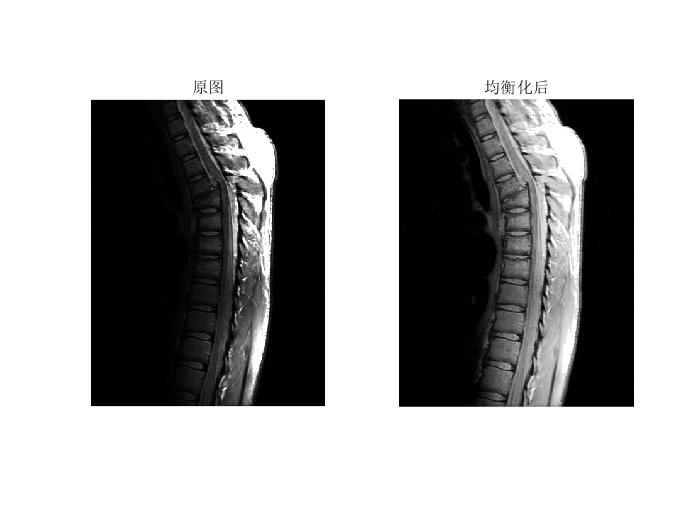
\includegraphics[width=0.9\linewidth]{figures/test3.JPG}
			\caption{code1:原图与直方图均衡后图像}
		\end{minipage}
		\begin{minipage}{0.49\linewidth}
			\centering
			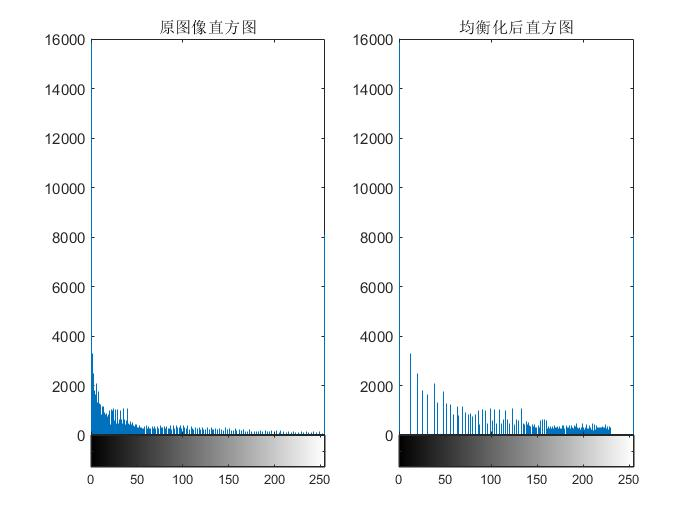
\includegraphics[width=0.9\linewidth]{figures/test4.JPG}
			\caption{code1:原图与直方图均衡后直方图}
		\end{minipage}
	\end{figure}
	导入图3.8(a),使用histeq函数,得到的原图像和直方图均衡后图像以及它们的直方图如下。从图像看,均衡化后图像细节更加明显,整体颜色更加明亮,但在黑色背景部分出现了一些噪点。从直方图看,直方图均衡化后总体上更加平均,但因为原直方图绝大部分像素值集中在0附近,所以直方图均衡后不能覆盖到像素值低的部分,高的部分可以正常近似平均。
	\begin{figure}[H]
		\centering
		\begin{minipage}{0.49\linewidth}
			\centering
			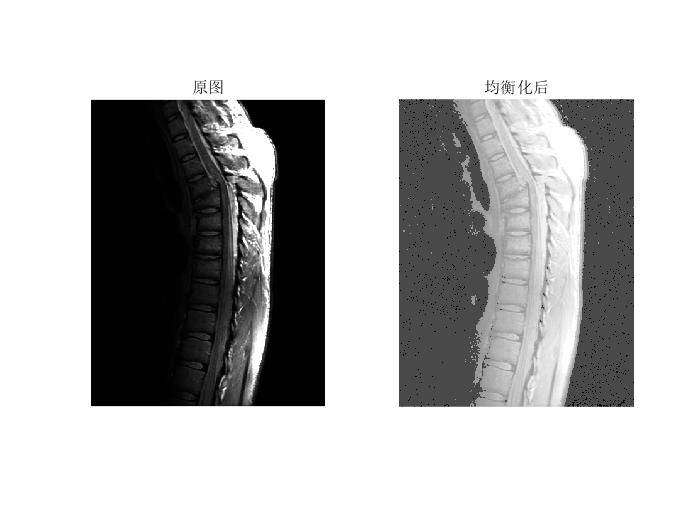
\includegraphics[width=0.9\linewidth]{figures/test1.JPG}
			\caption{code2:原图与直方图均衡后图像}
		\end{minipage}
		\begin{minipage}{0.49\linewidth}
			\centering
			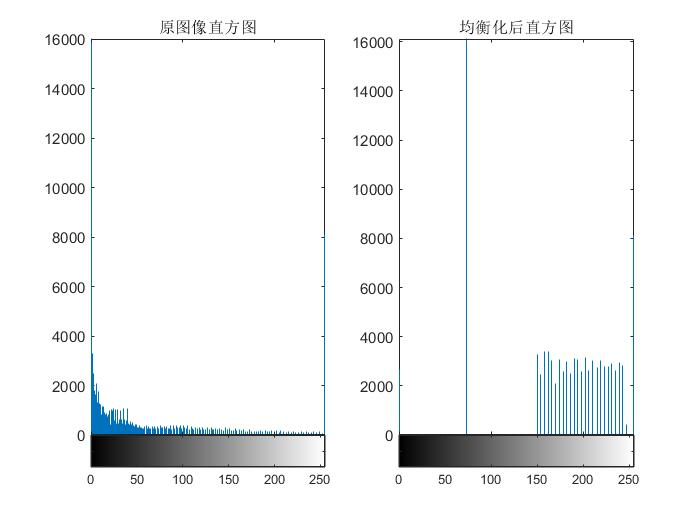
\includegraphics[width=0.9\linewidth]{figures/test2.JPG}
			\caption{code2:原图与直方图均衡后直方图}
		\end{minipage}
	\end{figure}
	\section{总结}
	本次实验的关键在于直方图的计算与直方图均衡的算法,直方图计算比较简单,只需要遍历图像的所有像素;直方图均衡也可以直接采用matlab的函数进行处理,但是最终结果并不理想。原始方法其实对这种像素值主要集中在0附近的直方图处理并不理想。之后参考了网上的另一算法,改变了映射关系,可以看到比较好地削减了某一像素值过高的情况。通过这次实验,我熟悉了数字图像处理操作的基础代码,因为是第一次接触图像处理,学习到了很多基本的matlab数字图像处理的函数。
\end{document}